\chapter{Data and Graphs chapter}

\section{Data Sources}

The data needed for constructing the dataset and performing the analysis come from multiple sources:
\begin{itemize}
    \item European Statistical Office (Eurostat) \cite{eurostat2022comext}
    \item World Trade Organization (WTO) \cite{wto2022stats}
    \item United Nations (UN) \cite{un2022population}
\end{itemize}

\subsection{COMEXT}

The starting dataset of my research is named COMEXT, and is published and maintained by Eurostat \cite{eurostat2022comext}. COMEXT is a statistical database for detailed statistics on international trade in goods\footnote{The definition of \textit{goods} provided by Eurostat is "\textit{all movable property including electricity}"}. It serves as an important indicator of the performance of the European Union (EU) economy, because it focuses on the size and the evolution of imports and exports of countries. It provides access not only to both recent and historical data of the EU and its individual Member States, but also to statistics of a significant number of non-EU countries. The information contained in it is based on data provided by the statistical agencies of the EU member states and trading partners.
Data are organized in tables, one for each year (or for each month) and each table contains information about the country that declared the transaction, the partner country, the product that was exchanged according to multiple international standard classifications (or nomenclatures), the value in euros of the exchange and its quantity in kilograms.
Let us now have a look at an extraction from this dataset, as you can see in Table \ref{tab:comextexample}.
\begin{landscape}
\begin{table}\label{tab:comextexample}
    \centering
    \resizebox{1.6\textheight}{!}{
\begin{tabular}{rrrrrrrrrrrrrrrrrrrr}
% \begin{tabular}{p{2.5cm}p{2.5cm}p{2cm}p{2cm}p{2cm}p{2cm}p{2cm}p{2cm}p{2cm}p{2cm}p{2cm}p{2cm}p{2cm}p{2cm}p{2cm}p{2cm}p{2cm}}
 \toprule
 DECLARANT & DECLARANT ISO & PARTNER & PARTNER ISO & TRADE TYPE & PRODUCT NC & PRODUCT SITC & PRODUCT cpa2002 & PRODUCT cpa2008 & PRODUCT CPA2 1 & PRODUCT BEC & PRODUCT SECTION & FLOW & PERIOD & VALUE IN EUROS & QUANTITY IN KG \\ \midrule
 61 & CZ & 4 & DE & I & 83023000 & 69915 & 2863 & 2572 & 2572 & 530 & 15 & 2 & 200101 & 284650 & 137370 \\
 5 & IT & 604 & LB & E & 85011010 & 71610 & 3110 & 2711 & 2711 & 410 & 16 & 2 & 200101 & 42089 & 11200 \\
 7 & IE & 5 & IT & I & 20021010 & 05672 & 1533 & 1039 & 1039 & 122 & 04 & 1 & 200101 & 97333 & 207000 \\
 4 & DE & 52 & TR & E & 85363030 & 77253 & 3120 & 2712 & 2712 & 420 & 16 & 2 & 200101 & 124054 & 3200 \\
 1 & FR & 720 & CN & E & 84823000 & 74630 & 2914 & 2815 & 2815 & 420 & 16 & 2 & 200101 & 18294 & 1300 \\
 30 & SE & 64 & HU & E & 72193310 & 67553 & 2710 & 2410 & 2410 & 220 & 15 & 2 & 200101 & 36002 & 18000 \\
 7 & IE & 720 & CN & E & 82089000 & 69561 & 2862 & 2573 & 2573 & 420 & 15 & 1 & 200101 & 15039 & 400 \\
 60 & PL & 1 & FR & I & 70091000 & 66481 & 2612 & 2312 & 2312 & 220 & 13 & 1 & 200101 & 12724 & 845 \\
 46 & MT & 400 & US & E & 85442000 & 77312 & 3130 & 2732 & 2732 & 220 & 16 & 1 & 200101 & 47203 & 0 \\
 30 & SE & 53 & EE & E & 62064000 & 84270 & 1823 & 1414 & 1414 & 620 & 11 & 1 & 200101 & 18944 & 500 \\
 1 & FR & 528 & AR & E & 90261099 & 87431 & 3320 & 2651 & 2651 & 410 & 18 & 2 & 200101 & 30657 & 500 \\
 3 & NL & 38 & AT & I & 28257000 & 52269 & 2412 & 2012 & 2012 & 220 & 06 & 2 & 200101 & 125073 & 20400 \\
 55 & LT & 5 & IT & I & 55103000 & 65187 & 1710 & 1310 & 1310 & 220 & 11 & 1 & 200101 & 26906 & 4033 \\
 5 & IT & 9 & GR & I & 84669195 & 72819 & 2940 & 2849 & 2849 & 420 & 16 & 2 & 200101 & 90529 & 5600 \\
 1 & FR & 4 & DE & I & 70140000 & 66595 & 2615 & 2319 & 2319 & 220 & 13 & 1 & 200101 & 410786 & 33400 \\
 5 & IT & 472 & TT & E & 94018000 & 82118 & 3611 & 3100 & 3100 & 410 & 20 & 2 & 200101 & 39182 & 25800 \\
 11 & ES & 75 & RU & E & 44091011 & 24830 & 2010 & 1610 & 1610 & 220 & 09 & 2 & 200101 & 27916 & 3000 \\
 61 & CZ & 3 & NL & I & 84807190 & 74918 & 2956 & 2573 & 2573 & 410 & 16 & 1 & 200101 & 167767 & 545 \\
 30 & SE & 39 & CH & E & 84563011 & 73113 & 2940 & 2841 & 2841 & 410 & 16 & 1 & 200101 & 295905 & 8500 \\
 32 & FI & 10 & PT & I & 48109190 & 64177 & 2112 & 1712 & 1712 & 220 & 10 & 2 & 200101 & 12252 & 13200 \\
 53 & EE & 54 & LV & E & 48229000 & 64291 & 2125 & 1729 & 1729 & 220 & 10 & 2 & 200101 & 14994 & 18678 \\
 6 & GB & 720 & CN & E & 84615011 & 73177 & 2940 & 2841 & 2841 & 410 & 16 & 1 & 200101 & 20997 & 1900 \\
 5 & IT & 60 & PL & E & 85189000 & 76492 & 3230 & 2640 & 2640 & 420 & 16 & 2 & 200101 & 250280 & 73200 \\
 5 & IT & 400 & US & E & 97020000 & 89620 & 9231 & 9003 & 9003 & 610 & 21 & 2 & 200101 & 12861 & 500 \\
 6 & GB & 61 & CZ & E & 84148079 & 74319 & 2912 & 2813 & 2813 & 410 & 16 & 2 & 200101 & 37962 & 2900 \\
 91 & SI & 5 & IT & I & 82074030 & 69564 & 2862 & 2573 & 2573 & 420 & 15 & 1 & 200101 & 17573 & 227 \\
 38 & AT & 92 & HR & E & 21032000 & 09842 & 1587 & 1084 & 1084 & 122 & 04 & 2 & 200101 & 17346 & 20200 \\
 1 & FR & 5 & IT & I & 39173231 & 58140 & 2521 & 2221 & 2221 & 220 & 07 & 1 & 200101 & 86548 & 29200 \\
 4 & DE & 52 & TR & E & 39173231 & 58140 & 2521 & 2221 & 2221 & 220 & 07 & 2 & 200101 & 75198 & 14400 \\
 6 & GB & 628 & JO & E & 84189990 & 74149 & 2923 & 2825 & 2825 & 420 & 16 & 2 & 200101 & 16498 & 10000 \\
 11 & ES & 4 & DE & I & 28129000 & 52241 & 2413 & 2013 & 2013 & 220 & 06 & 1 & 200101 & 17184 & 1800 \\
 8 & DK & 400 & US & E & 28183000 & 52266 & 2413 & 2013 & 2013 & 220 & 06 & 1 & 200101 & 140360 & 100000 \\
 4 & DE & 3 & NL & I & 82022000 & 69551 & 2862 & 2573 & 2573 & 420 & 15 & 1 & 200101 & 91395 & 3800 \\
 4 & DE & 63 & SK & E & 60012100 & 65512 & 1760 & 1391 & 1391 & 220 & 11 & 2 & 200101 & 48420 & 4200 \\
 92 & HR & 5 & IT & I & 94019080 & 82119 & 3611 & 3100 & 3100 & 220 & 20 & 1 & 200101 & 23887 & 10559 \\
 6 & GB & 8 & DK & I & 42029291 & 83199 & 1920 & 1512 & 1512 & 620 & 08 & 1 & 200101 & 73806 & 3100 \\
 11 & ES & 5 & IT & I & 85153100 & 73735 & 2940 & 2790 & 2790 & 410 & 16 & 1 & 200101 & 578296 & 29500 \\
 3 & NL & 386 & MW & E & 09024000 & 07414 & 0113 & 0127 & 0127 & 112 & 02 & 1 & 200101 & 97484 & 65000 \\
 17 & BE & 732 & JP & E & 39032000 & 57291 & 2416 & 2016 & 2016 & 220 & 07 & 1 & 200101 & 25108 & 5400 \\
 11 & ES & 3 & NL & I & 08103030 & 05794 & 0113 & 0125 & 0125 & 112 & 02 & 1 & 200101 & 16854 & 6200 \\
 1 & FR & 3 & NL & I & 72042900 & 28229 & 2710 & 3811 & 3811 & 210 & 15 & 2 & 200101 & 59015 & 258300 \\
 4 & DE & 979 & QZ & E & 29211930 & 51451 & 2414 & 2014 & 2014 & 220 & 06 & 2 & 200101 & 381600 & 372300 \\
 6 & GB & 17 & BE & I & 30021091 & 54163 & 2442 & 2120 & 2120 & 220 & 06 & 1 & 200101 & 4166599 & 1500 \\
 7 & IE & 6 & GB & I & 85421360 & 77641 & 3210 & 2611 & 2611 & 420 & 16 & 2 & 200101 & 438109 & 0 \\
 1 & FR & 640 & BH & E & 84431990 & 72659 & 2956 & 2899 & 2899 & 410 & 16 & 1 & 200101 & 41257 & 300 \\
 11 & ES & 3 & NL & I & 72193410 & 67554 & 2710 & 2410 & 2410 & 220 & 15 & 1 & 200101 & 118787 & 59300 \\
 7 & IE & 220 & EG & E & 84733090 & 75997 & 3002 & 2620 & 2620 & 420 & 16 & 2 & 200101 & 184452 & 1500 \\
 3 & NL & 388 & ZA & E & 90261051 & 87431 & 3320 & 2651 & 2651 & 410 & 18 & 2 & 200101 & 48644 & 900 \\
 1 & FR & 30 & SE & I & 84733010 & 75997 & 3002 & 2620 & 2620 & 420 & 16 & 2 & 200101 & 1138762 & 3800 \\
 60 & PL & 94 & YU & E & 16042090 & 03716 & 1520 & 1020 & 1020 & 122 & 04 & 2 & 200101 & 14171 & 9900 \\
 \bottomrule
\end{tabular}
}

    \caption{Random sample taken from the COMEXT dataset referring to imports and exports exchanged during January 2001.}
\end{table}
\end{landscape}
The data available follow the shown format. Each row corresponds to a transaction, an exchange of a certain good between two countries in a given period. The information available about each transaction is summarized here\footnote{ISO stands for International Standardization Organization, which harmonizes codes and abbreviations across the world (\url{www.iso.org}). The conversion is displayed in Appendix Table \ref{tab:iso2}.}:
\begin{itemize}
    \item \textit{DECLARANT} and \textit{DECLARANT ISO}: code and ISO name of the country that declared the trade.;
    \item \textit{PARTNER} and \textit{PARTNER ISO}: code and ISO name of the country with which the declarant traded;
    \item \textit{TRADE TYPE}: indicates whether the exchange was among two EU countries (I) or one was extra-EU (E);
    \item all the \textit{PRODUCT} columns: they are used to classify the good that was exchanged, according to different nomenclatures and standards;
    \item \textit{FLOW}: indicates whether the exchange was reported as an import (1) by the declarant or as an export (2);
    \item \textit{PERIOD}: indicates the time period of the exchange, in the format \texttt{yyyymm}\footnote{If it refers to a whole year then the format is \texttt{yyyy52}.};
    \item \textit{VALUE IN EUROS}: indicates the monetary value of the exchange between countries of that product;
    \item \textit{QUANTITY IN KG}: indicated the weight in kilograms of the exchange between countries of that product.
\end{itemize}



\subsubsection{Summary statistics}
Thanks to COMEXT data, we are able to conduct many types of analyses on commerce among countries. A first look at the data tells us that, by exploiting the variables that we have at disposal, we can observe if there are any trends in the EU economy as a whole, aggregating on all countries and products. This is shown in Figure \ref{fig:totaleu}. 

\begin{figure}
    \centering
    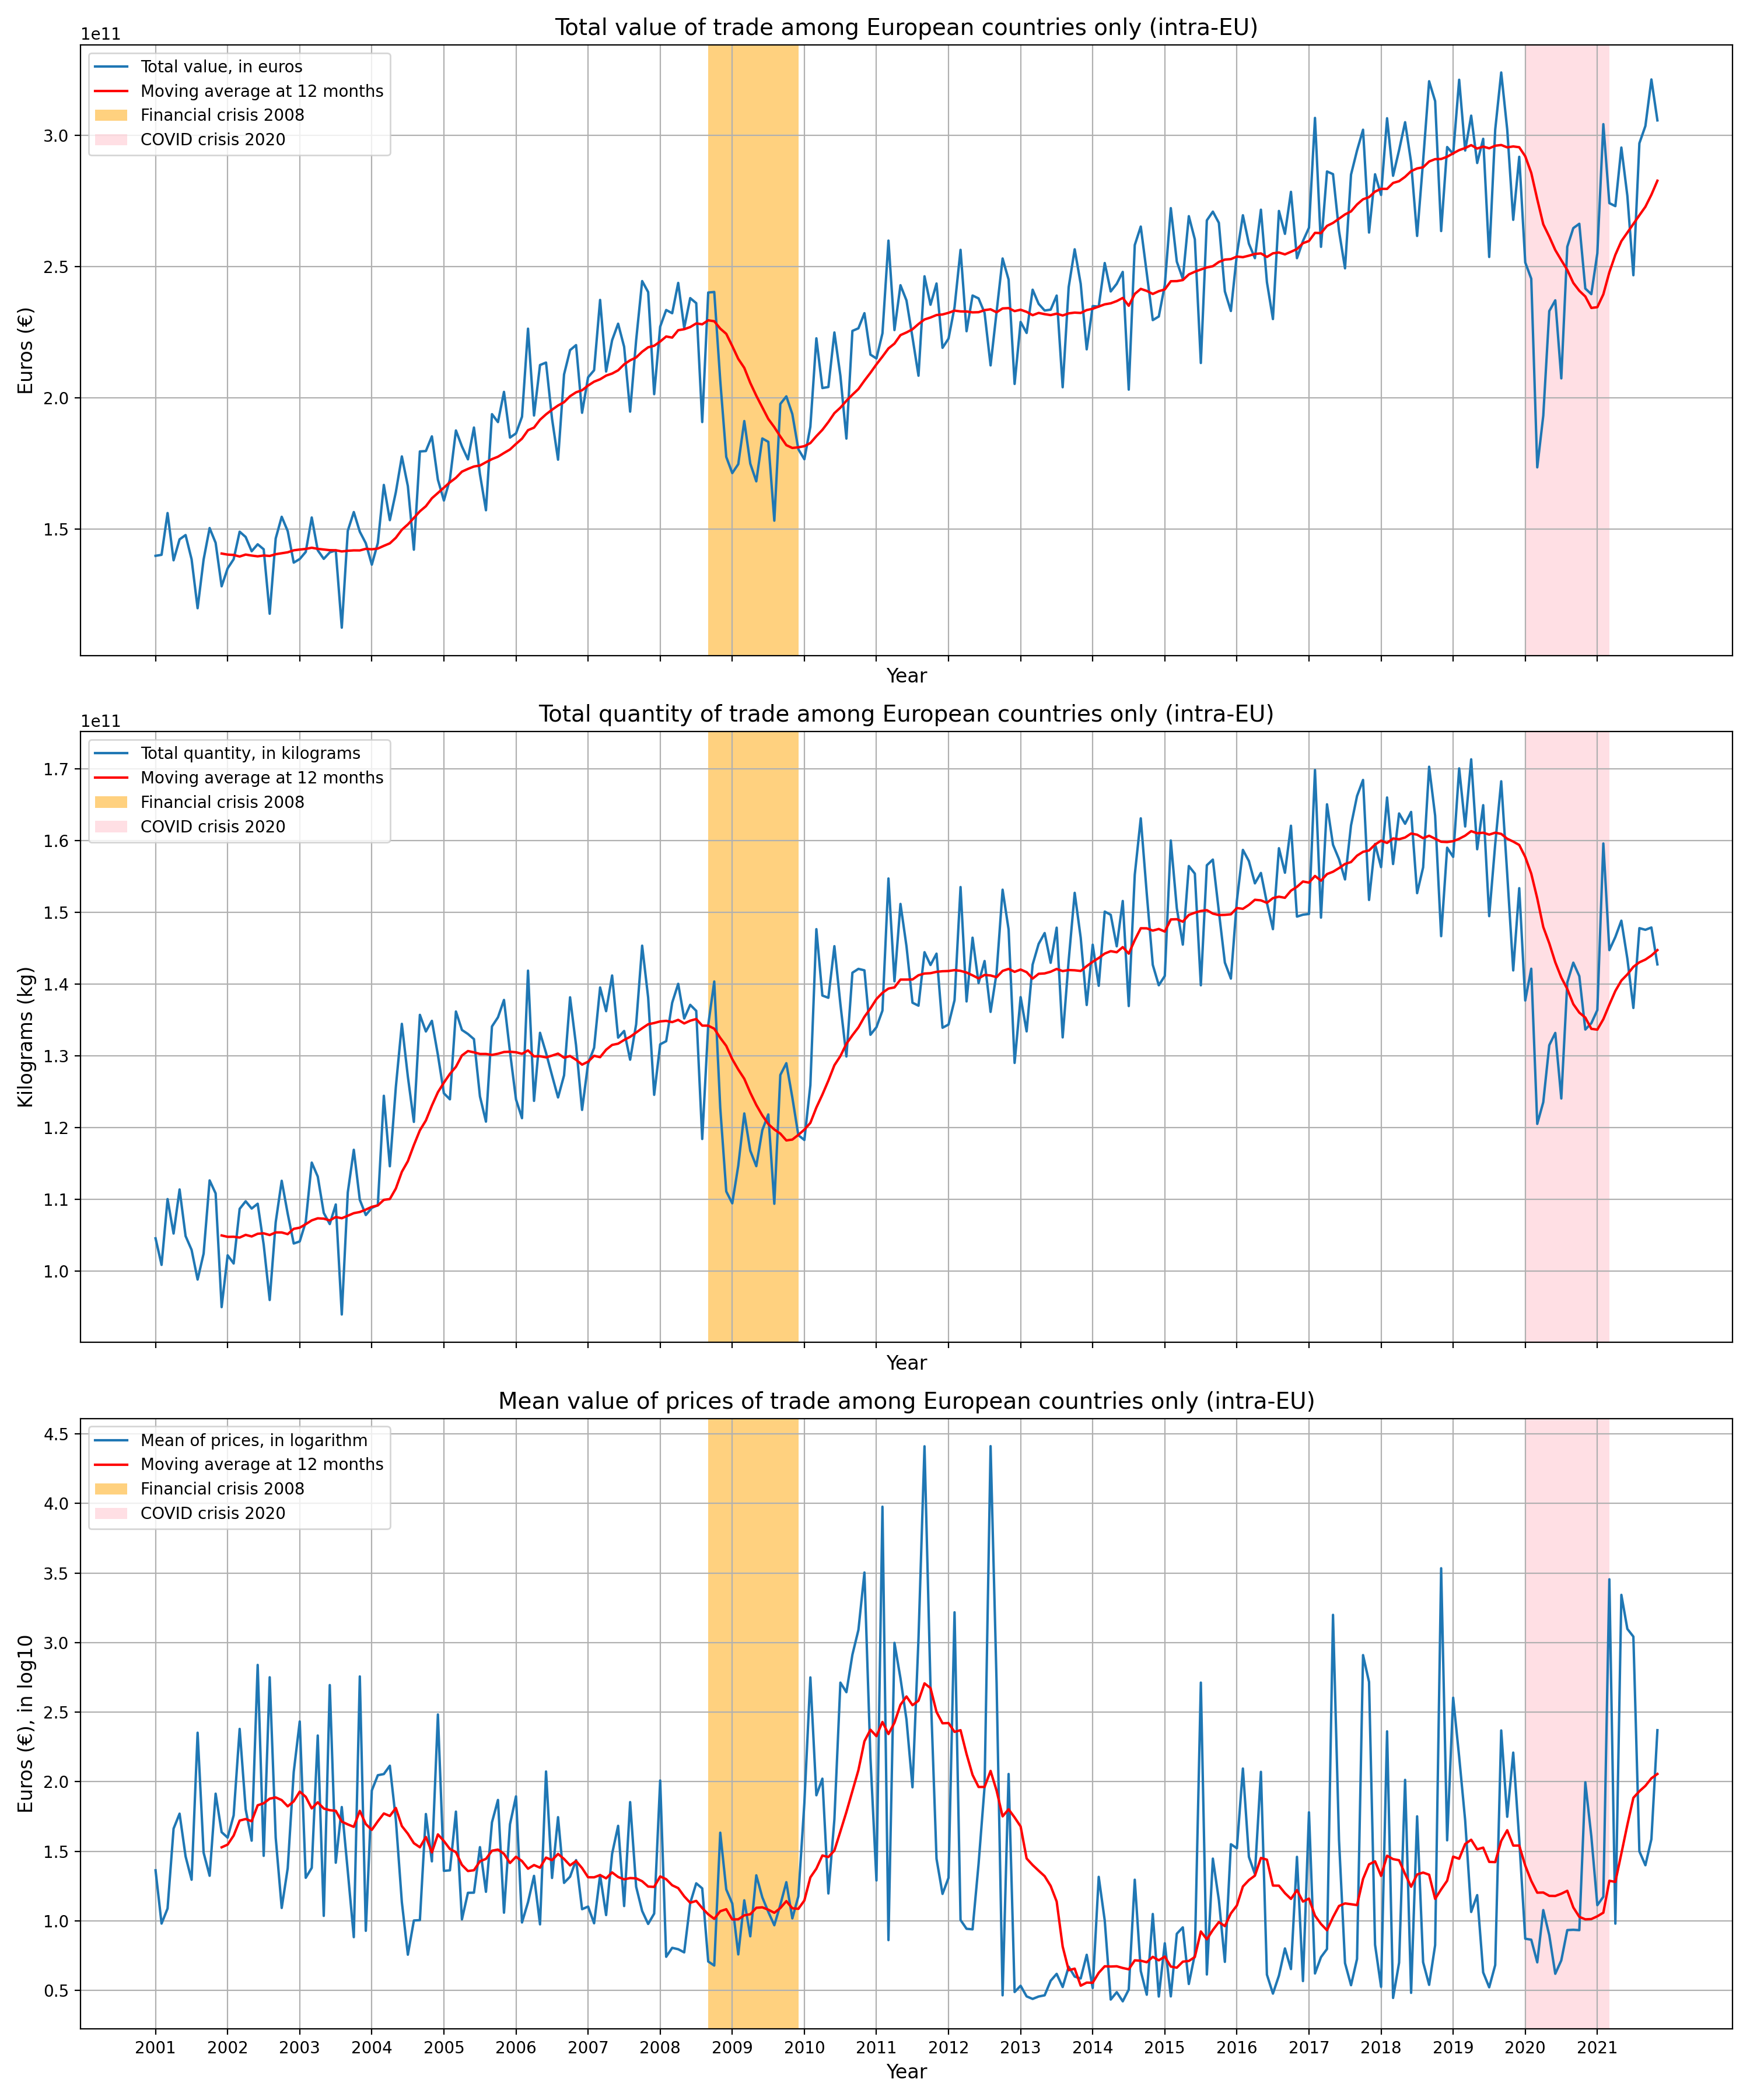
\includegraphics[width=\textwidth]{pics/TOTAL_VQP_INTRA.png}
    \caption{Long term trends of trade exchanges across EU member countries, by various indicators: (1) value (€), (2) quantity (Kg), (3) price (€/kg).}
    \label{fig:totaleu}
\end{figure}

In the first plot, we have on the horizontal axis time in years, while on the vertical axis we have monetary value expressed in euros. What is shown here is an aggregated sum of the total value of products exchanged by EU countries among themselves (intra-EU trade). This can be interpreted as an important indicator of the state of the whole economy, and in fact we can recognize in it two of the major economic events that happened in the last two decades: the 2008 financial crisis and the 2020 COVID-19 epidemic and related economic fallout. Since 2004 the growth of intra-EU trade was stable and sustained, up until the second semester of 2008, where we see a notable drop in total value, and a reprise only after the end of 2009. A similar effect can be seen at the beginning of 2020, where the lockdown due to the epidemic caused a sudden drop in the commerce of non-essential products, which almost brought the economy to a halt. Then production reprised in the second half of 2020, and we need to wait until 2021 for the values to reach pre-COVID levels.
If we look instead at the big picture, we see that overall intra-EU trade follows a positive trend that has basically doubled the value in 20 years. One has to wonder whether this increase in total money exchanged in commerce is due to an actual increase in production and circulation of goods, or is due just to inflation and higher prices of products. If we look at the second plot, we can observe the total quantity in kilograms of products exchanged in the EU economy. As before, we see a positive trend in the last 20 years, supporting our hypothesis that production has expanded. We also observe the same drops of trade exchanges following the two crises. Furthermore, what can be observed in both of the previous two plots is a yearly seasonality of these time series, where the values usually go up in the first trimester of the year, then they go down after mid-year, only to pick up again in the last part of the period. 
At last, in the third plot we see the evolution of prices in the same time frame, obtained by dividing each exchange's value by its quantity. Note that the vertical axis is in log scale. Here we can see a different behavior than previously. While in the first eight years of the millennium prices of traded products have been going down, with less and less volatility year by year (which can also explain why demand and commerce of these goods has gone up), we can easily see that in the period following the 2008 crisis they went rapidly up again. This is a known and reasonable effect of those events, since when dealing with scarcity and uncertainty prices naturally rise, and with them also variability. It took more than three years after 2009 for these inflated prices to go down, and it can be easily seen that by the start of 2014 they were even lower than before 2008. Then they started slowly to grow, as we observe a  slight positive trend until 2020, with periodical cycles which last about a year. After 2021, which marked a first step out of the pandemic with the diffusion of COVID vaccines, we see the economy picking up again, and as with the aftermath of crises, also prices and volatility increase.

%%esempio di tabella che viene da COMEXT -- altrimenti così son solo parole
%%Questo può essere quello che ti avevo segnato come capitolo 3 -- spiegazione etc etc 
%%Descrizione e visualizzazione del dataset - dati nulli, dati non comuni

\paragraph{COMEXT Data collection}
Historically, the main source of information about trade transactions between countries are customs authorities, which provide detailed information on exports and imports of goods with a geographical breakdown.
The COMEXT system was conceived and implemented in the early 90's,  following the adoption of the European Single Market on 1993, when customs formalities between Member States were removed. Since then, it has been continuously adapted and re-engineered to take into account technological evolution and new users' needs. The data gathered are based on two data collection systems:
\begin{itemize}
    \item data on trade in goods with non-EU countries are collected by customs authorities and are based on the records of trade transactions in customs declarations;
    \item data of intra-EU exchanges are directly collected from trade operators once a month.
\end{itemize}


The COMEXT dataset, however, presents a problem if one wants to use it to build an analysis on world trade. In fact, the only data contained in it are the ones reported by European countries, or even less than that, members of the European Union. Therefore, if we look at the whole network of commerce, we are missing some relevant information: the trade of extra-EU countries among themselves, since they have no obligation to communicate to Eurostat their records.
For this reason, and because I want to conduct a complete analysis and have a complete overview of the trade network, I needed to find another source of information, which I then integrated with COMEXT.

\subsection{WTO}
Similar to Eurostat, also the World Trade Organization (WTO) collects data about the global commerce of products among countries \cite{wto2022stats}. Data are periodically sent to the organization from member countries, hence the dataset contains information about all the major world countries. 
Mamaaooooooo

\section{Nomenclatures}

In order to classify products into categories, many nomenclatures have been published by different organizations that try to organize merchandise items in groups with similar features, so that aggregate statistics and analysis can be produced. One of them is the Classification of Products by Activity (CPA), maintained by the European Commission and Eurostat.
According to Eurostat \cite{eurostat2022website}, "\textit{a statistical classification or nomenclature is an exhaustive and structured set of mutually exclusive and well-described categories, often presented in a hierarchy that is reflected by the numeric or alphabetical codes assigned to them, used to standardize concepts and compile statistical data}".
This procedure ensures that data is comparable between EU Member States, and for the purposes of this research, it enables us to put together reports of exchanges declared by different countries.


